\documentclass[a4paper,twoside,11pt]{article}
\usepackage{a4wide,graphicx,caption,subcaption,fancyhdr,amsmath,amssymb,tabularx,array,cite,tabto,float, url,hyperref }
\usepackage[linesnumbered]{algorithm2e}

%----------------------- Macros and Definitions --------------------------

\setlength\headheight{20pt}
\addtolength\topmargin{-10pt}
\addtolength\footskip{20pt}

\newcommand{\N}{\mathbb{N}}
\newcommand{\ch}{\mathcal{CH}}

\fancypagestyle{plain}{%
\fancyhf{}
\fancyhead[LO,RE]{\bfseries\large Eindhoven University of Technology}
\fancyhead[RO,LE]{\bfseries\large 2ID26 Web Information Retrieval}
\fancyfoot[LO,RE]{\bfseries\large Department of mathematics and computer science}
\fancyfoot[RO,LE]{\bfseries\thepage}
\renewcommand{\headrulewidth}{1pt}
\renewcommand{\footrulewidth}{1pt}
}

\pagestyle{fancy}{%
\fancyhf{}
\fancyhead[RO,LE]{\bfseries\large Eindhoven University of Technology}
\fancyhead[LO,RE]{\bfseries\large 2ID26 Web Inforamtion Retrieval}
\fancyfoot[LO,RE]{\bfseries\large Department of mathematics and computer science}
\fancyfoot[RO,LE]{\bfseries\thepage}
\renewcommand{\headrulewidth}{0pt}
\renewcommand{\footrulewidth}{0pt}
}

%-------------------------------- Title ----------------------------------

\title{\vspace{-\baselineskip}\bfseries Google+ Search Engine}
\author{
    Alexander Nieuwenhuijse (0744933) \and
    Christian Stevandy (0870945) \and
    Fakhri Affif (0857457)\and
    Joelian Samuel (0872415)\and
    Marcelo Almeida (0877394)\and
    Youcef Mammar (0873972)
}
\date{\today}

%--------------------------------- Text ----------------------------------

\begin{document}
\maketitle
\raggedbottom
\section{Introduction}
introduction
\subsection*{Motivation}
The main motivation is to be able to query over Google+ users, finding interesting information about them. Using the techniques learned in the course, it is possible to infer a lot of things from the users based on their posts, communities, likes (called +1 in Google+) and more.

\subsection*{Goal}
The project goal is to have a search engine that is capable of research in the Google+ user database and retrieve relevant user profile and posts based on general interests, query by example and keywords.
\section{Architecture}
This section explains the overall architecture of the Google+ search engine and mentions used APIs and libraries.
\subsection*{Overall architecture}
\begin{figure}[h]
\begin{center}
    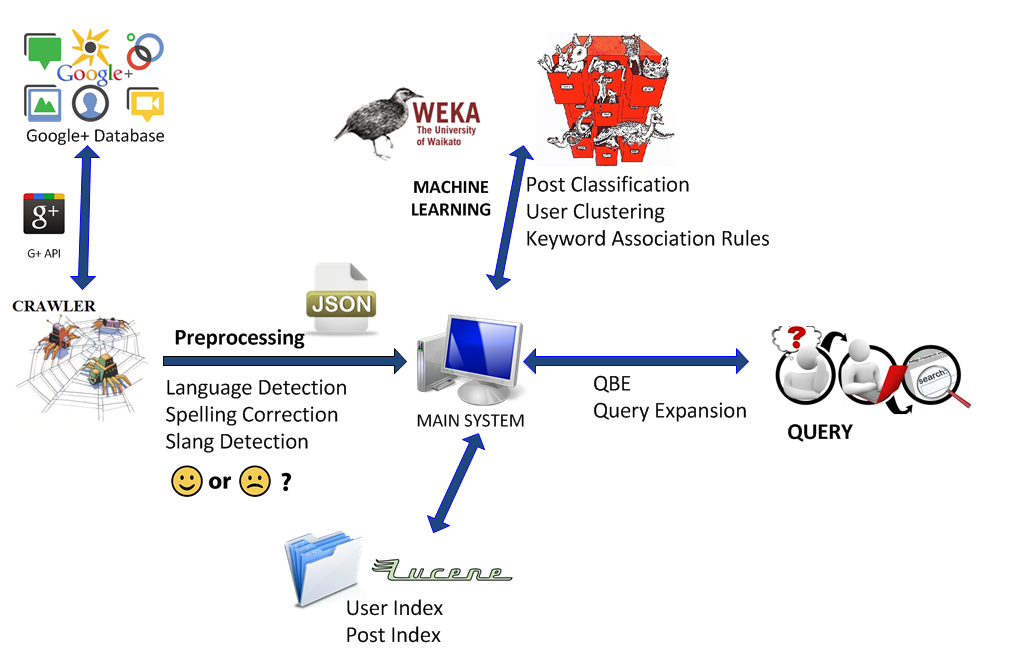
\includegraphics[scale=0.4]{images/architecture.png}
	\caption{Architecture sketch\label{architecture_sketch}}
\end{center}
\end{figure}
The architecture of the systems consist of a crawler that will get data from the Google+ database using the Google+ API. The output from the crawler is preprocessed with language and slang detection, spelling correction, and sentiment analysis. Preprocessed data is then used for machine learning, pattern mining and index building. The machine learning tasks consist of the training of classifiers and the clustering of user profiles. The queries can be processed with additional query by example and query expansion techniques.
\subsection*{Used API and Tools}
\subsubsection*{WEKA}
WEKA is an open source suite of machine learning algorithms. It contains tools for preprocessing, classification, clustering and other data mining related tasks. 
\subsubsection*{Apache Lucene}
Apache Lucene is an open source project, high performance, fully-featured text search engine library in Java. It includes an indexing and searching library that is suitable for making  a simple search engine.
\subsubsection*{Google+ API}
For the training and testing of our classifiers and for building a search engine, which can be queried by users, a large amount of data was required. To retrieve this data we used the Google+ Application Programmable Interface (API). This interface allows querying for Google+ posts and user profiles via web requests and returns an easy to parse result. The API is still under development by Google, and this provided some inconsistencies between the API specification and the results retrieved from our queries.
\subsubsection*{NLTK}
NLTK is a widely used library in the domain of human language processing which is written in Python. It can perform most of the operations one might need when working with a natural language, from sentence splitting to text classification. 
\subsubsection*{Alchemy API}
AlchemyAPI provides cloud-based text analysis infrastructure which can be used for various NLP related task. We used AlchemyAPI to extract the keywords from user posts, which are then used in keyword pattern mining. 
\subsubsection*{OpenNLP}
OpenNLP is a Java library for machine learning and processing of a text written in a natural language. For this task, it was used for tokenization and part-of-speech tagging.


%--------------------------------- IR ----------------------------------
\section{Information Retrieval Tasks}
\subsection{Crawler}
\textbf{Student Name: }Alexander Nieuwenhuijse \textbf{Student ID:} 0744933\\
In this subsection a description is given of the crawler that was created to retrieve Google+ posts, comments and user profile data. We start by motivating the use of the application programmable interface(API) provided by the Google+ followed by the implementation details of the crawler program and finish by showing the generated output that is used later on in the pipeline.
\subsubsection*{Motivation}
At the start of the project we decided that we wanted to make an offline search engine for posts, comments and user profiles on Google+. To realise this we need a large collection of data to fill our database such that most queries made by users will have corresponding documents in our database. It will not be possible for us to cover the entire Google+ collection of data due to time constraints and limitations on the interface used to retrieve documents. For the retrieval of documents we looked into two different sources: The Google+ API and the manually parsing of the Google+ web pages.
\subsubsection*{Problem formulation}
We want to retrieve post information and user profile data given a set of keywords or a specific Google+ community page and store this data in an easy to use format for the training of classifiers and to allow the building of an index on this data.
\subsubsection*{Approach}
When comparing both data sources we asked ourselves the following questions: "How much information does the source provide?", "How accurate is the provided data?", "What are the limitations of using this source?", "How much time does it take to mine the data?". When looking at the API we first noticed that it was very well documented and provided a very easy to learn interface. The result from querying the API was formatted in JSON which made parsing of the data almost trivial. The complete opposite was true when manually parsing the Google+ web pages. When looking at the source-code of a webpage displaying a list of posts made by a user we noticed a large piece of code that contained all the data of the posts displayed on the website, and some additional posts not shown on the website. These additional posts were part of some caching technique used by Google and would allow us to retrieve a lot more data from a single web requests than the API would. However, the problem with parsing the pages manually comes from the formatting, since the data cache is stored in an unknown JSON-like format without any specification. To use this data we would have to reverse-engineer the meaning of the data, which would be a very time consuming process. A comparison of the two data formats is given in the appendix.
Another major difference between the two sources is the accessibility. The API has restricted the number of requests allowed per day to 10,000 per user whereas the manually crawling of pages does not have a limit, since the probability of getting banned is very small if we do not brute-force the crawling process and we add some pauses between requests. Since we have access to six different API keys we should be allowed 60,000 requests per day. We expect to get about 5 posts per requests and 1 user profile per requests, which would result in 300,000 posts or 60,000 profiles. Not all of these posts or profiles will end up in our database since they are also subject to a language checker, and may not contain interesting content.
Due to the time constraints of this project we decided to use the API for our crawling tasks since it was easy to access and the request limitation should not hinder the retrieval of posts too much as we will only be presenting a proof-of-concept. However, if we were to develop a real search engine which should contain a larger data collection we would recommend writing a parser that parses the web pages, since these contain more information, some of which is not even supported by the API, and allow for faster data retrieval on a larger scale.

To retrieve the data from the Google+ API a crawler program was written in Python to create the web request, parse the results, check the language and spelling, and then write the data to disk for access by the next program in the pipeline. Since we wanted to label all the retrieved posts with a class we decided to download posts made to a specific Google+ community page. These community pages usually had one specific theme that could be classified into a bigger class, for example: All the posts retrieved from the community page of Samsung could be labeled as 'technology'. We required this labeling for the training and testing of our classifiers, which are introduced in section \ref{data_mining}.
Since the API is still being developed by Google the documentation does not always correspond with the implementation. We found out that the API was not properly supporting the retrieval of posts from community pages. In order to solve this problem we changed the retrieval of posts from community pages to the result of search queries. The API allows searching for posts containing specific words allowing us to create a list of search words and their corresponding class to label posts accordingly. So instead of retrieving posts from the Samsung community we search for posts containing the word Samsung and label these as 'technology'.
For every post found this way we also retrieve all the corresponding comments and label these the same way. After finding all the posts and their corresponding comments using a specified search word we retrieve all the profiles of the authors, and label these authors with the same label as the posts used to find this author. This way we can also classify authors based on their profile data. We noticed that the profile data provided by users was very diverse, sometimes all the data was provided and other times only a name and gender. This could cause problems for the classification process.

\textbf{Generated output}
For the classifiers to be trained and tested the output of the crawler is written to disk, which allows for easy filtering and separating of the data retrieved. Since we do not require all the data retrieved from the API when training and testing of the classifiers we apply some filtering within the crawler. For posts we are only interested in the user, the original content of the posts, a cleaned version of the content which does not include urls and smileys and we also store the derived sentiment using the technique explained in section \ref{sec:sentiment}. All the posts are stored in a JSON format such that the data can easily be imported by the classifiers. The same process is used for storing profile data.

\subsection{Query Expansion and Index Analysis}
\textbf{Student Name: }Marcelo Almeida \textbf{Student ID:} 0877394 \\
Introduction

\subsubsection*{Motivation}
In Information Retrieval (IR) a query is a way to materialize in a sentence (or word) the user's information needs. This means that if the query is poorly crafted, the user probably will not be able to retrieve the wanted content. One way to address the problem is to expand  the query by adding related terms, retrieving more results that might satisfy the information need. Here our goal is to do so relying on a dictionary, meaning that each query term will be mapped to a set of related terms and those terms will also be used to fetch the content from the database. Besides, the user expects this query to work fast, and that is usually done through an index. It is good to store this index occupying the least storage space as possible. We will also make a brief study of two index formats.

\subsubsection*{Problem formulation}
Given a query, we want to search for other words that have the same meaning of those used in the query. We also want to analyze how many KB the index occupies in known index implementations.


\subsubsection*{Approach}
Our first choice was to use an open source library for Python called NLTK (Natural Language ToolKit). It is built over Wordnet, which contains a well known set of synonyms, and have been in development for years. With this package we implemented the query expansion and also a way of using user feedback to change the meaning of the presented set of synonyms (relevance feedback). Unfortunately later we decided to build the interface using Java and we were not able to integrate these two programs. It was necessary to recreate the query expansion program in Java and we did so using a (Wordnet based) package from Apache Lucene project. This package did not offer the same functionality as the Python one and because of that, along with the time constraints, we could not add user feedback. In the end, the query expansion presents more terms related to those already used in the query.
 
For the study of the space usage we used two different types of index. First, using a Weka filter we converted the Reuters 50x50 dataset \cite{reuters50x50} to a vector space representation and built the adjacency matrix, represented by a CSV file. This file was rather sparse, as partially shown in Figure \ref{adjacency_matrix}.
\begin{figure}[h!]
 \centering
 \label{adjacency_matrix}
   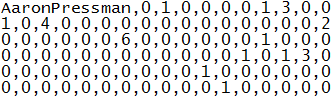
\includegraphics[width=0.5\textwidth]{adjacency_matrix.png}
 \caption{Only part of the adjacency matrix already shows its sparseness.}
\end{figure}

After that we created a Python program to build the inverted index of the same dataset (in three different ways, one of them using NLTK library to deal with the stopwords) and the comparison of all representations can be seen in the table \ref{space_comparison}).

\begin{table}[ht]
	\label{space_comparison}
	\centering
	\caption{Different types of index representations and their required storage space.}
    \begin{tabular}{| p{7cm} | p{3cm} |}
    	\hline
		Representation & Space requirements (KB) \\ \hline
		Usual adjacency matrix (CSV file) & 53.413 \\ \hline
		Inverted index without token normalization and \\ without removing stop words & 5.411 \\ \hline
		Inverted index without token normalization but \\ removing stop words & 4.785 \\ \hline
		Inverted index with token normalization (lowercase only) \\ and removing stop words & 4.567 \\ \hline
    \end{tabular}
\end{table}

\subsubsection*{Evaluation}
For the query expansion, we ran the same query with and without the expansion feature and we noticed that without context evaluation to use along with the dictionary it might be hard to know if the new (expanded) query means what the user wants. For example, a query for $\{mobile\}$ was expanded to $\{mobile, fluid, nomadic, peregrine, roving, wandering\}$. We get more results with the new query, but they will not be relevant to a user searching for mobile phone. It was not possible to calculate the recall, since we did not know how many documents were relevant (our database is too big for that evaluation). Regarding the precision, it would depend on the particular interest of the user. For the example above, if phone was the information need, the precision would be small. However, if it was movement, then it would be bigger.
For the index evaluation, it is very clear from the results presented in table \ref{space_comparison} that the inverted index is, indeed, a good choice as a data structure, occupying less than $ 9\% $ of the space used by the adjacency matrix.

\subsubsection*{Few observations}
We thought of a few possible different improvements that could also be interesting for query expansion. First, we could add different (smaller) weights for additional terms. That would make the original query more relevant but would still give a different result set. Second, instead of expanding the query without telling the user, we could show both the results for the query and also the other possible terms. Third (disregarding the dictionary), we could retrieve the results for the user’s query and extract the top keywords to show as suggestions. Since we did not intend to implement these ideas in the beginning and because of that they didn't fit in our timeframe.

\subsection{Spelling checker \& Slang-Detector}
\textbf{Student Name: }Joelian Samuel \textbf{ ID:} 0872415\\
This subsection describes the spelling checker and slang detector function which were used in raw data preprocessing.
\subsubsection*{Motivation}
A spelling-checking function is needed to increase accuracy when constructing vector for piece of text. Meanwhile, there are some words that will be considered as a typographical error whereas it is a valid word since it is a slang word. Therefore, besides a spelling checking function, the system also needs slang-detector function to check whether a word is categorized as either a typographical error or just a slang word.
\subsubsection*{Problem formulation}
Given a text, the system will try to correct all the mistyped words in that text before passing it to the next process within the pipeline.
\subsubsection*{Approach}
This function was built using Python. We created a class called spellCheck that contains both the spell-checking function and the slang-detector. Figure~\ref{fig:spellprocess}  depicts the process flow from input text unto clean content. 
\begin{figure}
\centering
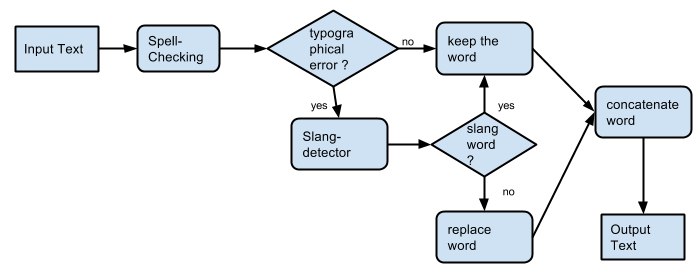
\includegraphics[scale=0.5]{images/spellprocess.png}
\caption{Spelling Checking Process Flow}
\label{fig:spellprocess}
\end{figure}
For the spell-checking and replace-word function, we are using a Python library called PyEnchant. Pyenchant supports many libraries for many languages such as Aspell, Ispell, Myspell, Uspell, Hspell, etc. These libraries are needed to make PyEnchant a generic spell-checking library for many languages. Since, our text will be in English, we only use the Aspell libraries from PyEnchant. Basically, for the spell-checking function, it is boolean retrieval since it will check to find the exact word in dictionary. And for the replacing-word, PyEnchant uses the Levenshtein Distance. Levenshtein Distance is a distance between two string. This distance can be obtained by counting the minimum number of several operations needed to transform one string to another i.e substitution, insertion, deletion of one character, or transposition two adjacent character. \\
For the slang-detector, we are using the API from Urban Dictionary. Besides the common slang word\footnote{taken from Wikipedia : Slang is represented as a lexicon of non-standard words and phrases within a language, typically associated with the subversion of a standard variety} such as ‘lol’, ‘brb’, or ‘lmfao’, this slang-detector also check whether the words is name of product like Samsung, iPhone, or name of places since those kind of words do not appear in the dictionary. Why Urban Dictionary is selected, because it is a dictionary that relies on user contributions. It makes Urban Dictionary becomes the most complete and reliable dictionary for  slang word since slang word can quickly change and increase in term of number. Like spell-checking, this function is also  boolean retrieval.  \\
\subsubsection*{Evaluation}
Given an input text that contains some typographical error  we check the result text to see if the mistake was corrected by the system. Table~\ref{tabelvalspell} shows examples of input and output as produced by our system. From these results we conclude that the function has run correctly.\\ 
\begin{table}[H]
   \resizebox{\textwidth}{!}{
    \begin{tabular}{|l|l}
    \hline
    Input Sentence                                                           & Output sentence                                                      \\ \hline
    Check out the latest PlayStation 4 commercial                            & Check out the latest PlayStation 4  commercial                       \\ \hline
    I say ''I'm always on'' is because I have a sleep disorder i never sleep & I say I m always on is because I have a sleep disorder i never sleep \\ \hline
    \end{tabular}
}
    \caption {Example result of evaluation}
    \label{tabelvalspell}
\end{table}



\subsection{Data labeling and cleansing}
\textbf{Student Name: }Youcef Mammar \textbf{Student ID:} number\\

On Google+ users can label their posts explicitly through \#hashtags to make it easy to retrieve 
all the posts related to an event, topic or tv program. And when they don’t use hashtags, 
scanning the keywords inside each post can return precious information about its subject.

\subsubsection*{Motivation}
The motivation is to use the hashtags and some keywords to label the posts into normalized categories 
in order to allow searching and classification based on a subject.

\subsubsection*{Problem formulation}

\subsubsection*{Approach}
We create categories and give each a set of related keywords. A keyword can be either a regular word of 
the post, or a hashtagged word. Then we use a quite straight forward boolean retrieval technique to 
feed a dictionary of categories which for each category, indexes the related posts. \\
The categories and their related keywords are store in a csv file of this architecture:

\begin{verbatim}
 iphone|technology
 android|technology
 bmw|automotive
 ...
\end{verbatim}

The detection relies on the spell checking as a preprocessing step. As we deal with social content, it is 
best to lowercase everything, ignoring acronyms and proper nouns. We think that users are usually careless 
about conserving the case of such words on social media.

\subsubsection{Evalutation}



\subsection{Building the index}
	\textbf{Student Name: }Christian Stevandy \textbf{ID:} 0870945\\\\
	This section describes how the post index are build and how the post retrieved from a query in the index.
\subsubsection*{Motivation}
	User post contains a lot of interested information. People can retrieve information in a post by giving a query in our search engine. In order to answer a query from a user it is required to make index for user posts.
\subsubsection*{Problem formulation}
	Given a collection of posts in JSON representation and a query from user. The posts are used for building index. Query from user retrieves information from the index.
\subsubsection*{Approach}
	We built the index from posts that are generated by the crawler. The query is handled using boolean retrieval and vector space model representation and also created our user post database for offline use.\\\\
	\textbf{a. Building the Index} \\\\
	The index is implemented by using the library Lucene. The user posts generated by the crawler are stored in this Lucene index: \\\\\\\\\\\\\\\\
	\begin{figure}[h]
		\begin{center}
			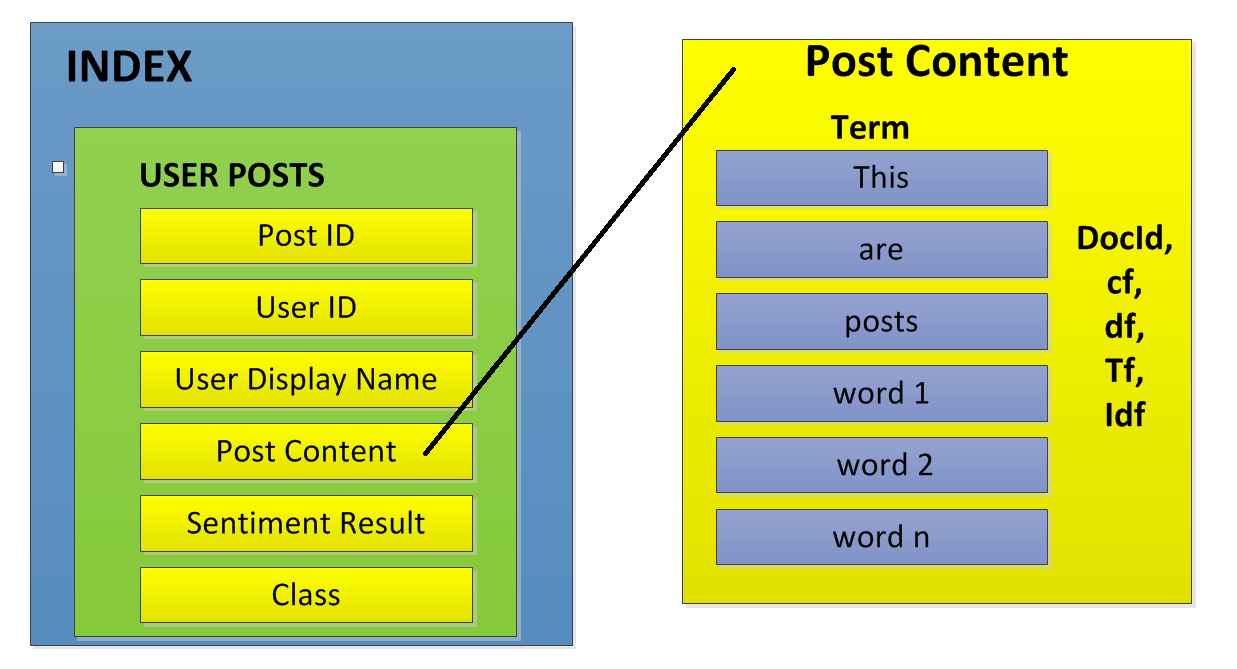
\includegraphics[scale=0.4]{images/postindex.png}
		\caption{Post Index\label{post_index}}
		\end{center}
	\end{figure}
	\\Figure~\ref{post_index} consist of multiple fields. One of its fields is Post Content, this field represent a text of a user post which is contains an inverted index and documents vector space model.\\\\
	\textbf{b. Searching Index}\\\\
	Searching is implemented using Lucene with boolean query and vector space model techniques.\\
	\\
	\textbf{Boolean Query}\\
		-  OR query is processed by unioning term’s posting list in index.\\
		-  AND query is processed by intersecting term’s posting list in index.\\
	\\
	\textbf{Scoring Document}\\
	In vector space model, user posts are represented in a collection of string vector. For example, a post ��This is a post�� will be represented as string vector (This,is,a,post).
	The retrieved user posts are ranked based on how high their score are. Score is calculated using cosine similarity in vector space model.\\
	\begin{figure}[h]
		\begin{center}
			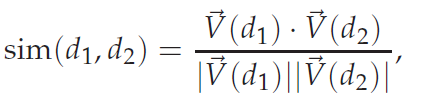
\includegraphics[scale=0.4]{images/cosinesim.png}
		\caption{Cosine Similarity Equation\label{cosinesim}}
	\end{center}
	\end{figure}

\subsubsection{Evaluation}
Evaluation is done manually by giving a query and evaluates the result. Index should be built first before testing a query. A test query is given by giving a Boolean ‘OR’, ‘AND’. The query result is listed by their rank so it is conclude this task is satisfying.


% TODO XXX ADD A TASK

%--------------------------------- DM ----------------------------------
\section{Data Mining Tasks}
\subsection{Naïve Bayes Classifier}
\textbf{Student Name: }Alexander Nieuwenhuijse \textbf{Student ID:} 0744933\\
This subsection describes the technique used for building a naïve bayes classifier and how it was used within the project.
\subsubsection*{Motivation}
We want to be able to classify posts based on topics such as “technology”, “Entertainment” etc. This can then be used to query for posts with the same topic and help disambiguation of a user query.
\subsubsection*{Problem formulation}
To be able to classify posts into a predefined set of tasks we use training data generated by the crawler and use this data to train a naïve bayes classifier. This classifier can then be used to determine topics for a user query and help with the building of an index on the data generated by the crawler.
\subsubsection*{Approach}
The technique used for building a Naïve Bayes classifier is relatively easy when compared to other classification techniques, and it classifies its input very reliably. It is a probabilistic classification technique that, given a set of attributes and classes, will determine which class has the highest probability of describing an input document based on its attributes. It is important to note that this technique assumes independence between the attributes for every class.
The naïve bayes classifier classifies a document that has the highest probability:$ P(C|Document-terms)$. Using Bayes theorem this is equal to:
$$P(C|Document-terms)= \frac{P(Document-terms|C)P(C)}{P(Document-terms)}$$ 
To estimate the value of $P(Document-terms|C)P(C)$ we use a labeled training set of data which contains a set of Document-terms and their corresponding class. Given this training set (T) we estimate the following probability:
\begin{eqnarray*}
P(C|Document-terms) & = & P(T_{1}|C)\cdot P(T_{2}|C)\cdot\ldots\cdot P(T_{n}|C)\\
 & = & \sum_{i=1}^{n}P(T_{i}|C)\:\text{}\{Assuming\, independence\}
\end{eqnarray*}
The probability of $P(T_{i}|C)$ is determined as follows: 
$$P(T_{i}|C)=\frac{T_{ct}}{\sum_{t'\in V}T_{ct'}}$$ 
where $T_{ct}$ is the total number of occurrences of the term $T_{i}$ in the set of training documents with class $C$.
We can estimate $P(C)$ using the following estimator: $$P(C) = \frac{N_{c}}{N}$$ where $N_{c}$ is the number of documents with class $C$ in the total training set.
Using these probabilities we can determine the class which has highest probability of a document belonging in that class.
\subsection{Support Vector Machine Classifier}
\textbf{Student Name: }Name \textbf{Student ID:} number\\
Introduction
\subsubsection*{Motivation}
motivation
\subsubsection*{Problem formulation}
problem formulation
\subsubsection*{Approach}
approach

\subsection{Nearest Neighbor Classifier}
\textbf{Student Name: }Name \textbf{Student ID:} number\\
Introduction
\subsubsection*{Motivation}
motivation
\subsubsection*{Problem formulation}
problem formulation
\subsubsection*{Approach}
approach

\subsection{User Classification}
\textbf{Student Name: Joelian Samuel }Name \textbf{ID:} 0872415\\
This subsection contains the explanation for query by example feature which was build using classification and clustering techniques.
\subsubsection*{Motivation}
Having a search engine for determine user similarity is an interesting feature for a social media. The similarities can be found from the topic of interest, gender, location, hobby, job  or relationship status for example. For this task, the motivation is to classify user data using Google+ user's attribute into several classes and used this classification model to get friends recommendation for other user.
\subsubsection*{Problem formulation}
Having a set of user data, we should be able to determine what data mining technique is appropriate to classify user and also to build a class model for this data.
\subsubsection*{Approach}
Since user data don't have any predefined class, we should use clustering technique in order to get the class for each user. Broadly speaking, there are four sub-processes to be undertaken to achieve the objective of this task. Figure~\ref{fig:usercluster} shows us the connection between sub process.
\begin{figure}[H]
	\centering
	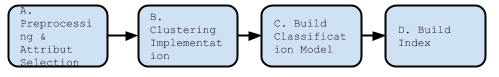
\includegraphics[scale=0.7]{images/usercluster.png}
	\caption{User Clustering Process Flow}
	\label{fig:usercluster}
\end{figure}

\subsubsection*{Pre processing \& Attribute Selection}
Google+ provides its users with many attributes. However, some users do not use them. In fact, there are  few users that do not use any of these attributes at all. Therefore, as a first step of this task, we decided to use two most used attributes : Gender and Relationship Status, also we used one attribute to get user interests : About Me.

For 'About Me'� attribute, we did a weighting for each word using TF-IDF technique. After we got TF-IDF score for each word, we picked 77 words that have the highest value assuming that words were spread evenly over our data set. These words would represent the interest of user so we called it 'Interest Words'�. After this process, every user would have 79 attributes. In order to determine a value for every 'Interest Words'�, we did a simple scanning through every user's About Me attribute and check whether it contained one of the 'Interest words'�.  if so, we gave score 1 and 0 otherwise and this was the end of this sub process.  After this process, we would have a new dataset of users with 79 attributes each.

\subsubsection*{Clustering Implementation}
The new set data of user from sub process A would be used in this sub process. We choose K-Means technique for this part since it was the simplest clustering technique. K means aims is to cluster n data into k clusters in which every data belongs to cluster with the nearest mean. For this task, we used WEKA tools and the parameters that we used are :\\
\begin{enumerate}
	\item Distance Function = Euclidean Distance
	\item Maximum Iteration = 100
	\item Num Cluster       = 15
	\item Seed              = 100
\end{enumerate}
After this process, every user data would be completed with cluster data.  Table~\ref{percentageuser} shows  distribution every cluster. \\
\begin{table}[H]
 \centering
    \begin{tabular}{|l|l|l|l|l|l|}
    \hline
    Cluster & Percentage  & Cluster & Percentage & Cluster & Percentage  \\ \hline
    0       & 153 ( 2 \%)  & 1       & 353 (5 \%)  & 2       & 4674 (64 \%) \\ \hline
    3       & 7 ( 0 \% )   & 4       & 341 (5 \%)  & 5       & 275 (4 \%)   \\ \hline
    6       & 50 ( 1 \%)   & 7       & 20 (0 \%)   & 8       & 35 (0 \%)    \\ \hline
    9       & 842 (12 \%)  & 10      & 53 (1 \%)   & 11      & 31 (0 \%)    \\ \hline
    12      & 114 ( 2 \%)  & 13      & 90 (1 \%)   & 14      & 235 (3 \%)   \\ \hline
    \end{tabular}
    \caption {Summary of Class}
    \label{percentageuser}
\end{table}
The complete result for this process can be seen in Appendix. \\

\subsubsection*{Build Classification Model}
After sub process B, we again get a new data set. We want to build class model using classification technique so that any new user can be classified into certain class using this model and the technique that we choose was Random Tree. Random Tree is a way to form decision tree by choosing random edge weights. This task also is done by WEKA tools and level of accuracy by using this technique achieves 94.8 \%. The complete result for this process can be seen in Appendix.

\subsubsection*{Create Index}
To improve search performance, the user data is indexed using Apache Lucene.

\subsubsection*{Evaluation}
Evaluation is done manually by trying to give a new user input that does not exist in the raw data and the system checks to see if the class that assigned to new user is match with the characteristics of the user. Some examples of data evaluation can be seen in Appendix.
\subsection{Sentiment Analysis}
\textbf{Student Name: }Youcef Mammar \textbf{Student ID:} 0873972\\

\subsubsection*{Motivation}
Sentiment analysis is becoming a popular area of research and social media analysis,
especially around user reviews or user interactions involving an opinion about a product
or a company. Identifying opinion polarity, while often not very accurate, is still very
useful and are particularly interesting for companies which want to receive direct (and free)
feedback from their clients.

\subsubsection*{Problem formulation}
Our crawler has gathered a big set of posts, some of them are explicitely related to a brand.
(like contain the username +Microsoft) or product names (like “Surface”). How can we
In the following we will explore some of the options we have to classify a set of posts.



\subsubsection*{Approach}

While there are many possible ways to approach the problem, they all involve some machine learning technique.

Our first try was to use a sentiment dictionary, which for a given words, for a given meaning (part of speech \&
context), could return a polarity score. However the results weren’t as good as expected. The main reason is we
could not easily determine the part of speech of a word or its context, and as we know, the polarity of a word can widely vary depending of theses.

For example, in theses two posts, the word “angry” carries two different meanings which a human can tell only by the context.
\begin{itemize}
 \item ``2 angry customers broke into an apple store last monday'': objective
 \item ``This swiping keyboard really makes me angry'': negative

\end{itemize}


The biggest problem in not being able to identify parts of speech is more visible when we deal with amplifiers
such as “really”. Not knowing which adjective this “really” is attached to makes it difficult to compute a global score for “... really makes me angry”.

Moreover, SentiWordNet didn’t include smileys as words, which could have been very interesting since smileys
express often unambiguously the emotions involved in a tweet.

We won’t go again through explaining how Naive Bayes works since there is a section dedicated to it. But we have
to say that we choose for the sake of simplicity to use a Bernoulli model, which we thought would not have a big
impact since we are dealing with reasonably short texts, where every relevant word (ie not a stop word) will usually appear only once.

The latter method surprisingly gave much better results, after training the classifier on 119783 labeled
sentences (some of them containing smileys). This set of data was obtained by mixing the manually crafted data sets:
“Stanford Sentiment Treebank” and a “twitter sentiment corpus” found on sananalytics.com.

Because our labeled data sets featured only positive and negative posts (no objective posts or any shades of theses),
we had to simplify and focus on 2 only possible classifications: positive and negative.

Input data (training and test data) is cleaned to get rid of irrelevant parts of the content such as punctuation,
misspelled words, urls, \#hashtags, @usernames (twitter) or +usernames (Google+). Also we removed stop words, as the
number of features tend to be very high with Bernoulli method, and working only with the most discriminative is likely
to improve the classification.

We also rely on the spellchecker to correct words such as “Awsuuuuuume”. Smiley and other common words of the internet
such as (“lol”, “haha”, ”arrgh”, etc) are detected and replaced with either the words “smily” or “angry” depending of their
meaning, then processed as regular words. All of this happens during the preprocessing phase.

Then we used Classify.NaiveBayes for the NLTK python package. As a technical detail, the processing of the trained data
(ie the classifier as a python object) is stored on the hard-drive once and for all to speed up the sentiment classification.

\subsubsection*{Evaluation}
We thought that the best way to evaluate our classifier is to try it on part of our labeled data.
We trained the classifier on 80\% of our labeled data set and tested it on the other 20\%.

If for example we want to query for positive posts, we reach then an accuracy of 75\%.

It is safe to say that the best sentiment analysis is done by humans\cite{sentiment_analysis}. However, according to a recent
study conducted at the University of Pittsburgh on Recognizing Contextual Polarity in Phrase-Level Sentiment Analysis\cite{polarity},
humans agree on sentiment only 80\% of the time.


\begin{figure}[h]
\centering
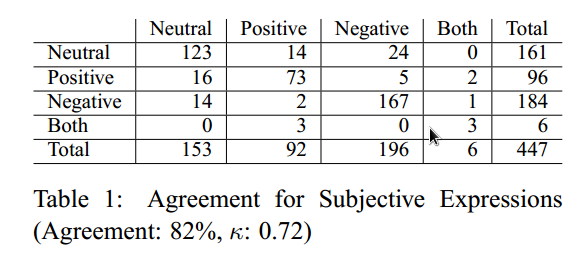
\includegraphics[scale=.5]{images/sent1.png}
\caption{This table is from the ``Recognizing Contextual Polarity in Phrase-Level Sentiment Analysis''}
\end{figure}

If we look now at the precision and the recall, we find

\begin{description}
 \item[For a positive query]

  precision: 0.908 and
  recall: 0.819


 \item[For a negative query]

  precision: 0.806 and
  recall: 0.899

\end{description}

We can see how precision for negative queries is lower than positive’s. We can explain it by looking at some of the negative posts.
Negations are often expressed using the word “not” but by basing our classifier only on words, we often miss this forms of negation.
For this reason, a sentence like “I’m really not happy with the new iPhone, it could be improved” could be evaluated to positive and be
ignored by the query. When a classifier doesn’t catch as much relevant content as it should, we say it has a low recall.

The same way, a sentence like “Trying out the nexus 5: not bad!” and other euphemisms which are very common in social talking, would be
evaluated to negative while it’s positive, leading to a low precision.

\begin{figure}[h]
\centering
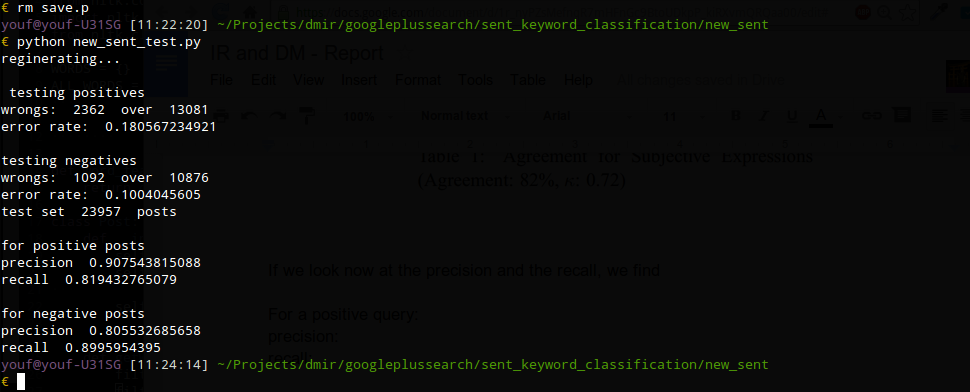
\includegraphics[scale=.4]{images/sent2.png}
\caption{This is the output of the test carried on 23 957 short text samples. It show the error rate and other performance figures}
\end{figure}



\subsubsection*{Some outlooks}
\begin{itemize}
 \item
 We could try to work around the bad recall for negative posts using a combination 2-grams and 1-grams as features. This would also help with adverbs that serve as adjective amplifiers.
\item
An even more robust approach could try to use grammar rules to extract the dependecies between the words, though it is arguable that such an approach would work on social media content, as the users tend to use poor grammar.
\item
he words case can contain important information about the emotion of a post as people tend to use caps to evoke anger or sometimes surprise. It certainly would have been an interesting feature if we had more than 2 classes (eg. very negative, negative, objective, positive, very positive). Unfortunately, our data set was limited in that regard.
\item
Bayesien classifiers are relatively very easy to implement and usually give good result with text but it would be interesting to see what we can have with other classifications methods, particularly SVM.

\end{itemize}



% TODO XXX ADD A TASK

%--------------------------------- Conclusion ----------------------------------
\section{Conclusion}
conclusion

%\bibliographystyle{unsrt}
%\bibliography{experimental_project_bib}

%--------------------------------- Appendix ----------------------------------
\section{Appendix}
\subsection*{Appendix A}
\begin{itemize}
	\item Summary of K-Means clustering result :
	\begin{table}[H]
    \begin{tabular}{|l|l|l|l|}
    \hline
    Cluster & Gender & Relationship Status & Most High Value “Interest Words”               \\ \hline
    0       & other  & single              & cars, community                                \\ \hline
    1       & male   & single              & science, school, games                         \\ \hline
    2       & male   & ~                   & -- (all words have low value)                  \\ \hline
    3       & male   & in a relationship   & consultant, engineer, manager, solutions       \\ \hline
    4       & male   & married             & wife, time                                     \\ \hline
    5       & male   & ~                   & marketing, technology, time                    \\ \hline
    6       & male   & ~                   & tech, technology, writer                       \\ \hline
    7       & male   & married             & family, life, technology                       \\ \hline
    8       & male   & ~                   & circle,s college, school, student, development \\ \hline
    9       & female & ~                   & life, staff, experts                           \\ \hline
    10      & female & single              & fashion, food, analyst, interests              \\ \hline
    11      & female & in a relationship   & passion, family, mom                           \\ \hline
    12      & male   & in a relationship   & geek, world, information                       \\ \hline
    13      & male   & ~                   & life,  world, time                             \\ \hline
    14      & ~      & ~                   & -- (all words has low value)                   \\ \hline
    \end{tabular}
	\end{table}
	\item Confusion matrix for Random Tree classification
	\begin{table}[H]
    \begin{tabular}{|l|l|l|l|l|l|l|l|l|l|l|l|l|l|l|l|}
    \hline
    A   & B   & C    & D & E   & F   & G  & H & I  & J   & K  & L  & M  & N  & O   & <- Classified as \\ \hline
    151 & 0   & 1    & 0 & 0   & 1   & 0  & 0 & 0  & 0   & 0  & 0  & 0  & 0  & 0   & A = Cluster 0    \\ \hline
    0   & 303 & 13   & 0 & 5   & 13  & 5  & 0 & 3  & 0   & 1  & 0  & 2  & 6  & 2   & B = Cluster 1    \\ \hline
    1   & 2   & 4652 & 0 & 2   & 15  & 0  & 0 & 1  & 0   & 0  & 0  & 1  & 0  & 0   & C = Cluster 2    \\ \hline
    0   & 0   & 0    & 6 & 1   & 0   & 0  & 0 & 0  & 0   & 0  & 0  & 0  & 0  & 0   & D = Cluster 3    \\ \hline
    0   & 9   & 6    & 1 & 285 & 22  & 3  & 1 & 1  & 4   & 0  & 0  & 2  & 5  & 2   & E = Cluster 4    \\ \hline
    0   & 7   & 58   & 0 & 7   & 182 & 5  & 1 & 2  & 5   & 0  & 0  & 0  & 7  & 1   & F = Cluster 5    \\ \hline
    0   & 1   & 4    & 0 & 3   & 5   & 36 & 0 & 0  & 0   & 0  & 0  & 0  & 0  & 1   & G = Cluster 6    \\ \hline
    0   & 0   & 3    & 0 & 4   & 2   & 0  & 7 & 0  & 0   & 0  & 1  & 0  & 2  & 1   & H = Cluster 7    \\ \hline
    0   & 0   & 0    & 0 & 0   & 3   & 0  & 0 & 32 & 0   & 0  & 0  & 0  & 0  & 0   & I = Cluster 8    \\ \hline
    0   & 1   & 5    & 0 & 10  & 6   & 0  & 0 & 0  & 814 & 0  & 1  & 0  & 5  & 0   & J = Cluster 9    \\ \hline
    0   & 9   & 0    & 0 & 4   & 0   & 0  & 0 & 0  & 6   & 34 & 0  & 0  & 0  & 0   & K = Cluster 10   \\ \hline
    0   & 0   & 0    & 0 & 5   & 0   & 0  & 1 & 0  & 6   & 0  & 14 & 4  & 1  & 0   & L = Cluster 11   \\ \hline
    0   & 2   & 5    & 0 & 1   & 3   & 5  & 0 & 1  & 0   & 0  & 1  & 93 & 2  & 1   & M = Cluster 12   \\ \hline
    0   & 0   & 2    & 0 & 4   & 8   & 2  & 3 & 0  & 1   & 0  & 0  & 0  & 70 & 0   & N = Cluster 13   \\ \hline
    0   & 4   & 1    & 0 & 4   & 9   & 1  & 0 & 0  & 0   & 0  & 0  & 0  & 0  & 216 & O = Cluster 14   \\ \hline
    \end{tabular}
\end{table}
\item Example of User Data to test User Clustering
\begin{table}
    \begin{tabular}{|l|l|l|l|}
    Gender & Relationship Status & Interest Word                                      & Class    \\
    female & ~                   & website development web  software services         & cluster9 \\
    male   & ~                   & sports games fish son father husband               & cluster2 \\
    male   & single              & web designer                                       & cluster1 \\
    male   & married             & politics science technology writer                 & cluster4 \\
    female & ~                   & web media writer technology consultant information & cluster5 \\
    \end{tabular}
\end{table}
\end{itemize}

\end{document}
